\documentclass[a4paper,10pt]{article}
\usepackage[utf8]{inputenc}
\usepackage{graphicx}
\usepackage{booktabs}
\usepackage{rotating}
\usepackage{subfigure}
\usepackage{caption}
\bibliographystyle{plos2009}%
%opening
\title{Text S2 -- Assessing the impact of taxon sampling on phylogeographic reconstruction} % aargh, lousy name
\author{
Luiz Max de Carvalho \\
\and Nuno Faria \\
\and Guy Baele\\
\and Andres Perez \\
\and Philippe Lemey \\
\and Waldemir Silveira 
}
\date{}
\begin{document}

\maketitle

\section{Background}
The data sets used in this study presented preferential sampling, with some countries being overrepresented.
Sampling bias constitutes an important concern \cite{Faria2012,Lemey2013,polar}
% A possibility, unexplored in this paper, is to sample each location with probability proportional to its disease prevalence
% In theory, a Bayesian approach should offer a certain degree of protection against model mispecification and sampling bias by bla bla...
\section{Comparing rate matrices}
Sometimes \\
L1 and L2 norms
We thank Professor Marc A. Suchard (UCLA) for advice on this topic.\\
\section{Quantifying spatial signal extraction}
KL root for each subsample \cite{KL}
\section{Bayesian Stochastic Search Variable Selection}
See Figures S\ref{sfig:bssvsA} and S\ref{sfig:bssvsO}. 
\section{Parameter estimation and demographic reconstruction without the overrepresented locations}
Additionally, we assessed the robustness of our temporal reconstruction by using only sequences from 2000 to present.
For this analysis, we used the Gaussian Markov Random Field (GMRF) smoothing prior on coalescent times, also known as 'skyride' model.
These results are presented in Figure~\ref{sfig:only2000sky}.
% TODO: more discussion on this 
%%%%%%%%%%%%%%%%%%%%%%%%%%%
\section{Parameter estimation with downsampling}
% For our experiments, we obtained five downsampled data sets for each serotype
\section{``Representation-informed'' priors}
\section{Results and Discussion}
%\newpage
\section*{Figure Legends}
\textbf{Figure S\ref{sfig:trade}. Exportation, importation and production time series for pigs, cattle and sheep in South america.} Panel A shows exportations in log(\# of heads) of live animals for pigs, sheep and cattle.
Panels B and C show importation and overall production (population increase), respectively.

\textbf{Figure S\ref{sfig:tradeinfo}. Kernel density estimation for the trade-informed priors used in this study.} Information on cattle, sheep and pigs trade was retrieved from FAO and used to create trade-informed prior distributions for the CTMC infinitesimal rate matrix.
Each prior was evaluated for prior predictive probability (marginal likelihood) using the PS and SS algorithms. 

\textbf{Figure S\ref{sfig:AvsO}. Scatterplot of estimated rate matrices for serotypes A and O} We plotted all overllaping rates (Serotype O without Paraguay) estimated using a symmetric CTMC model for both serotypes, to investigate whether the two serotypes have different spatial patterns.

\textbf{Figure S\ref{sfig:bssvsA}. Bayesian Stochastic Search Variable Selection for five downsampled subsamples of serotype A sequences} We performed the BSSVS analysis on five downsampled data sets (reduced Argentina representation) and plotted the results as in Figure 3 in the main text.

\textbf{Figure S\ref{sfig:bssvsO}. Bayesian Stochastic Search Variable Selection for five downsampled subsamples of serotype O sequences} We performed the BSSVS analysis on five downsampled (equal numbers of Ecuadorian and Colombian sequences) data sets and plotted the results as in Figure 3 in the main text.

\textbf{Figure S\ref{sfig:only2000sky}. Skyride coalescent reconstructions using sequences from 2000 to present only for both serotypes.}
As in the main text, disease cases and vaccination in doses per head are overlaid to the demographic reconstructions.


\newpage
\bibliography{Text_S2}
\newpage
\begin{center}
\begin{figure}[ht]
\begin{center}
\subfigure[A]{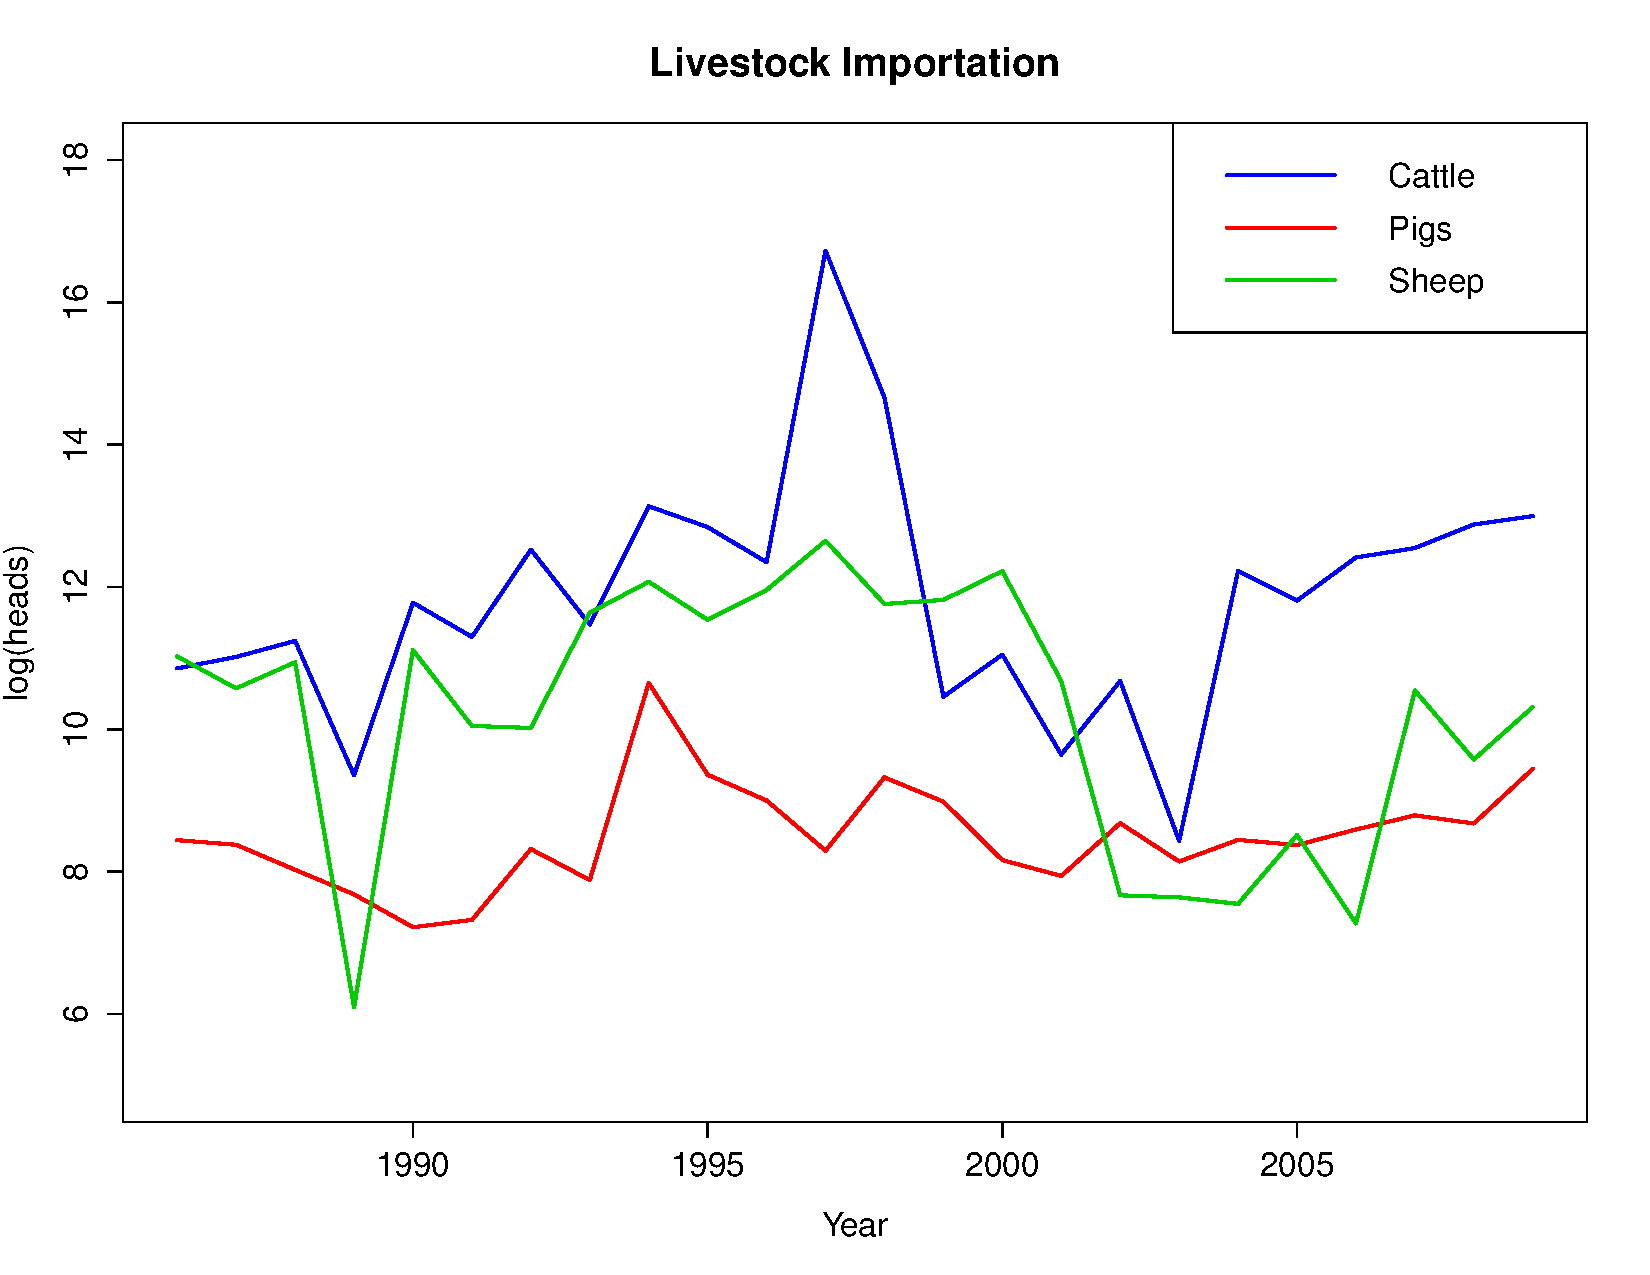
\includegraphics[scale=.250]{FIGURES/importation.pdf}}\\
\subfigure[B]{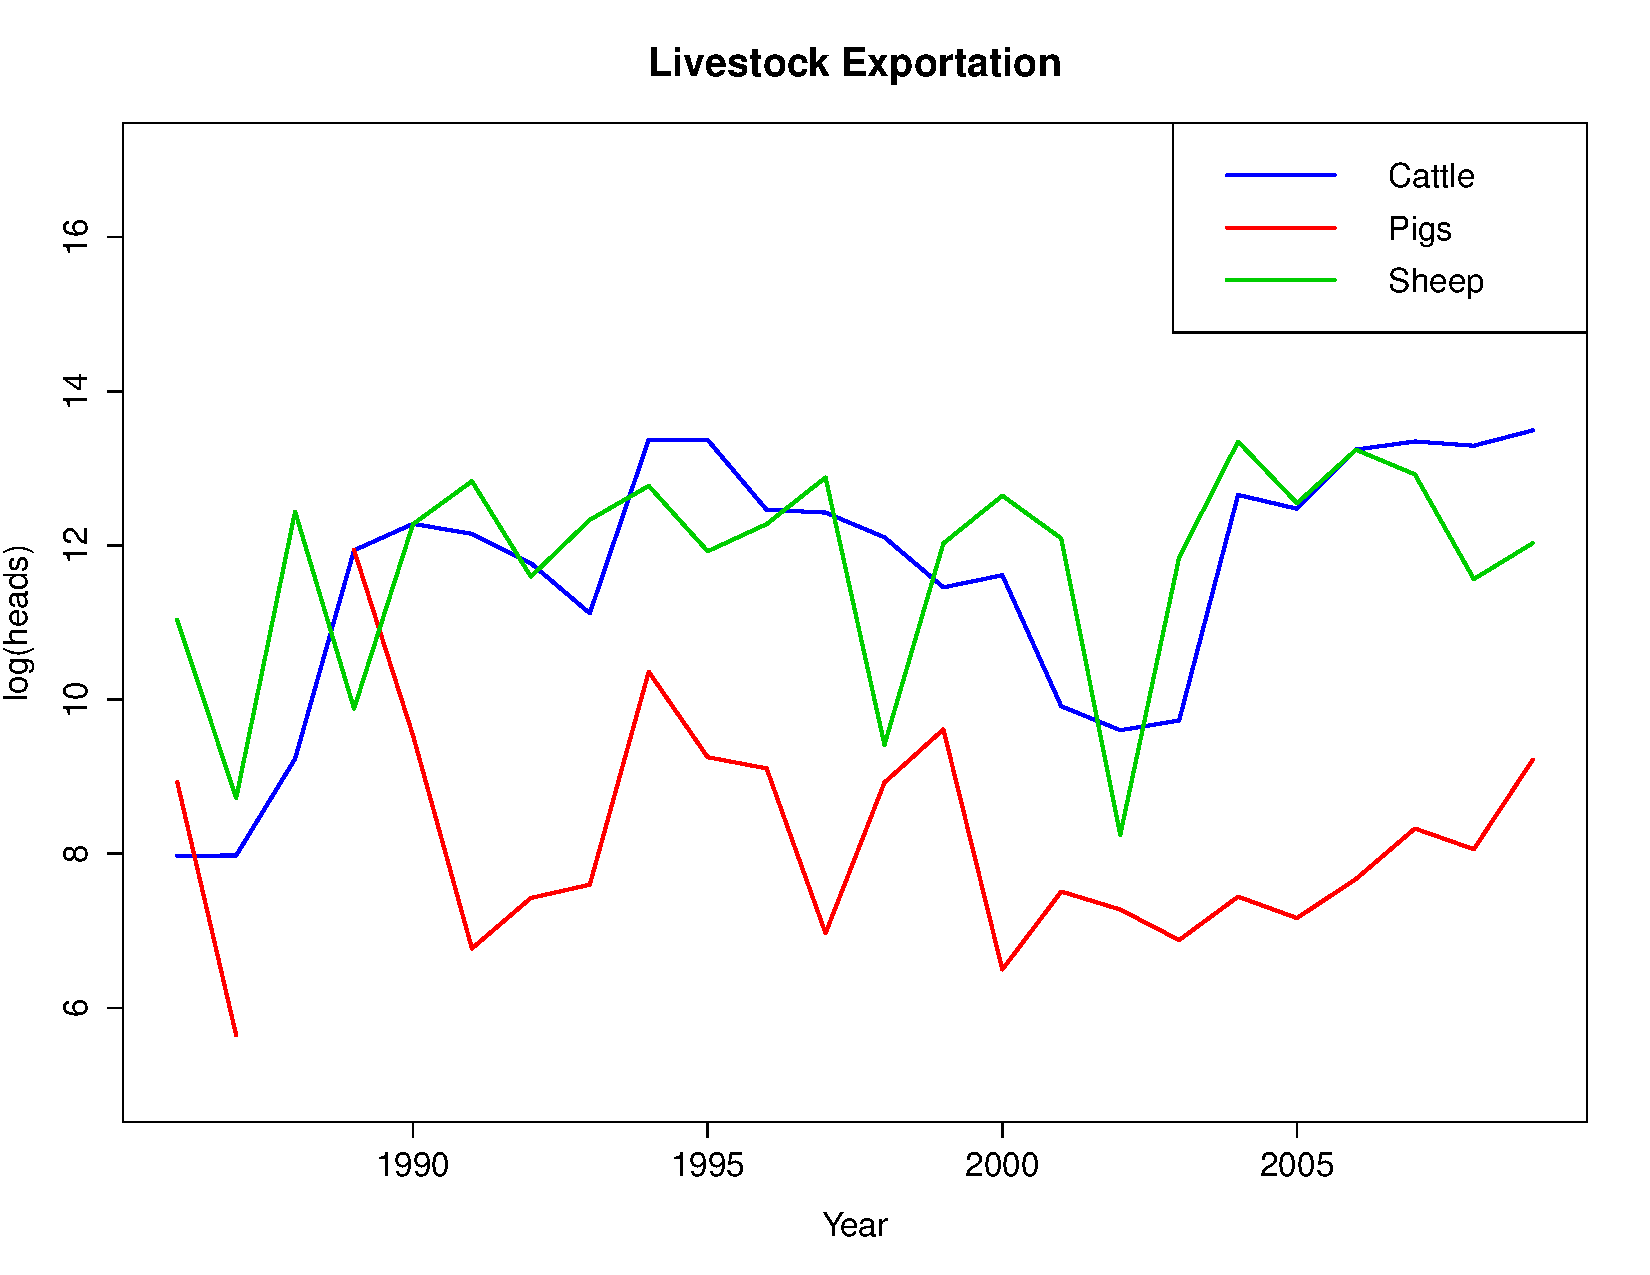
\includegraphics[scale=.250]{FIGURES/exportation.pdf}}\\
\subfigure[C]{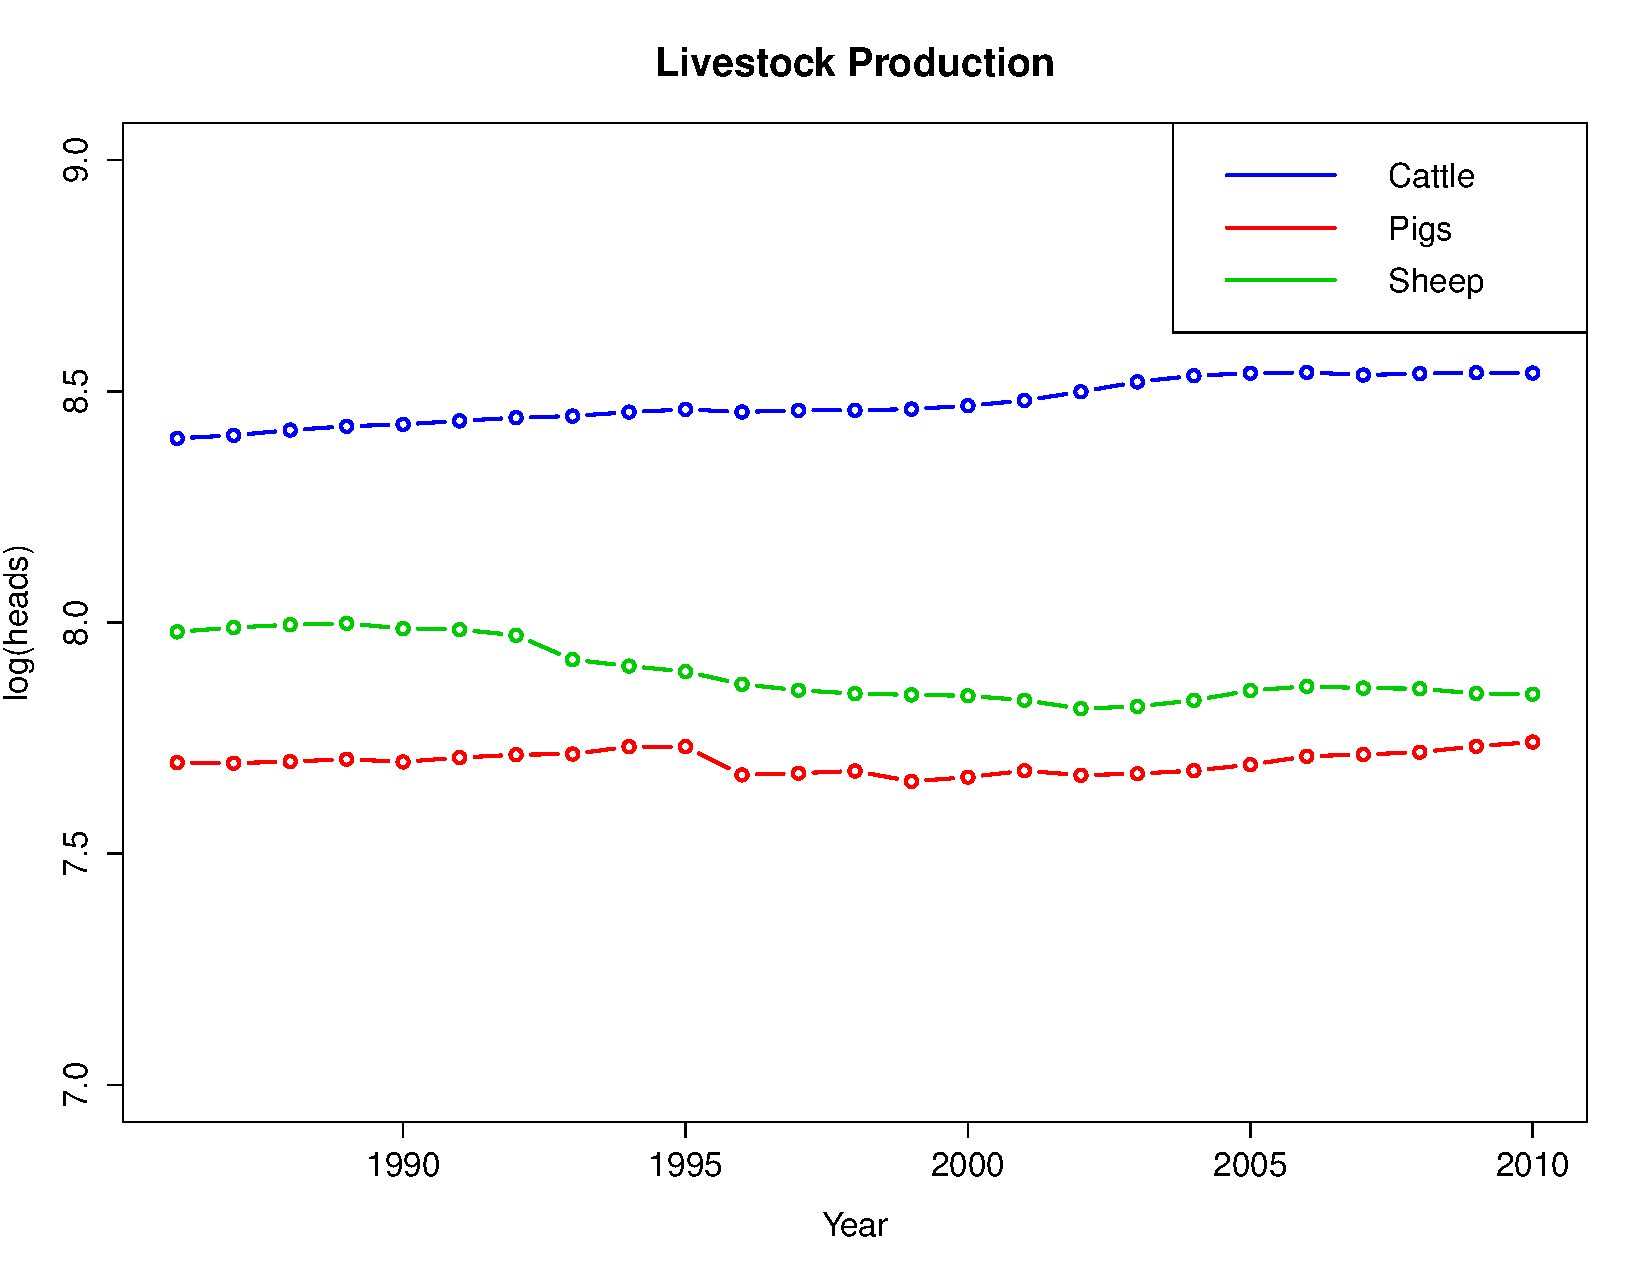
\includegraphics[scale=.250]{FIGURES/production.pdf}}
\end{center}
\caption{}
\label{sfig:trade}
\end{figure}
\end{center}
\newpage
\begin{figure}[ht]
\begin{center}
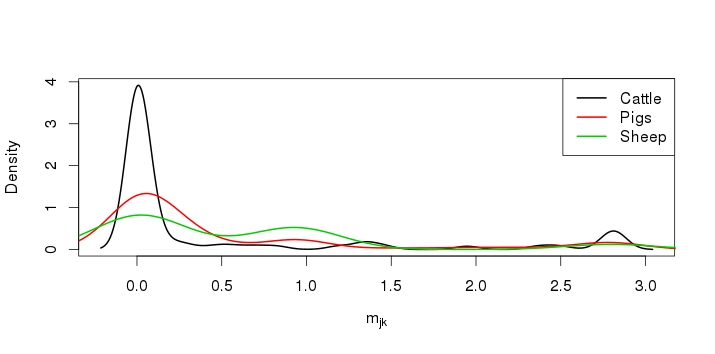
\includegraphics[scale=.5]{FIGURES/trade_info.jpeg}
\end{center}
\caption{}
\label{sfig:tradeinfo}
\end{figure}
\newpage
\begin{figure}[ht]
\begin{center}
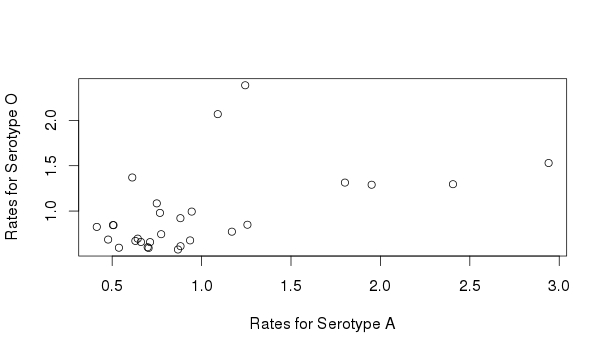
\includegraphics[scale=.5]{FIGURES/A_vs_O_symmetric.jpeg}
\end{center}
\caption{}
\label{sfig:AvsO}
\end{figure}
\newpage
\begin{center}
\begin{figure}[ht]
\subfigure[]{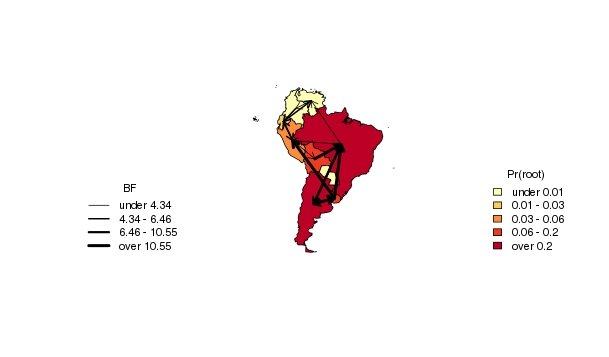
\includegraphics[scale=.450]{FIGURES/A_ss1.jpeg}}
\subfigure[]{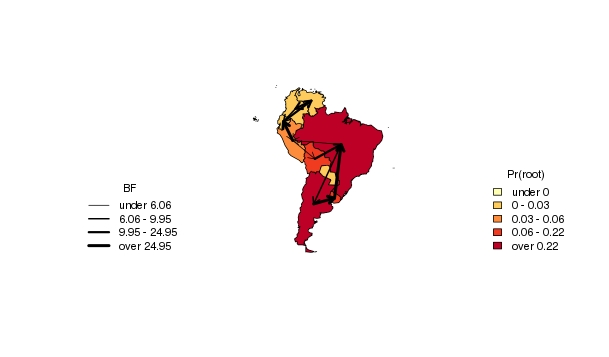
\includegraphics[scale=.450]{FIGURES/A_ss2.jpeg}}%\\
\subfigure[]{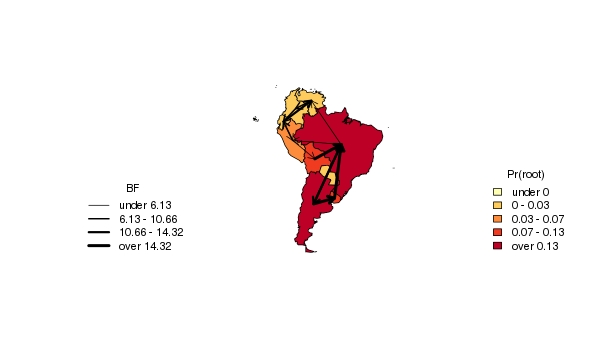
\includegraphics[scale=.450]{FIGURES/A_ss3.jpeg}}
\subfigure[]{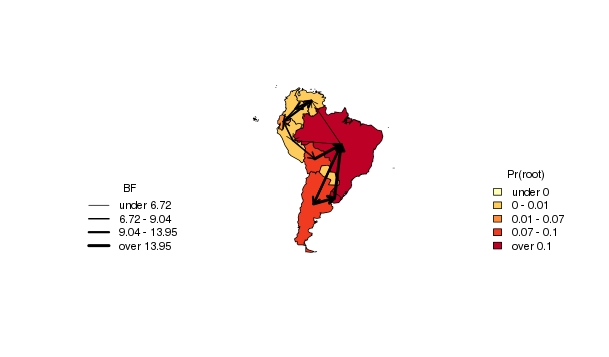
\includegraphics[scale=.450]{FIGURES/A_ss4.jpeg}}%\\
\subfigure[]{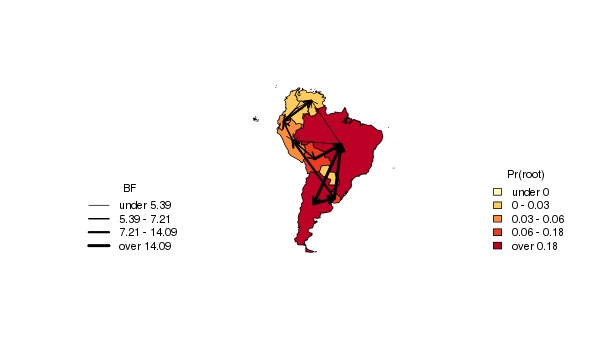
\includegraphics[scale=.450]{FIGURES/A_ss5.jpeg}}
\caption{}
\label{sfig:bssvsA}
\end{figure}
\end{center}
\newpage
\begin{figure}[ht]
\begin{center}
\subfigure[]{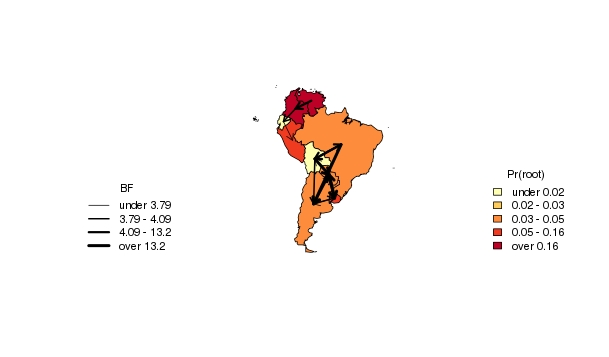
\includegraphics[scale=.450]{FIGURES/O_ss1.jpeg}}
\subfigure[]{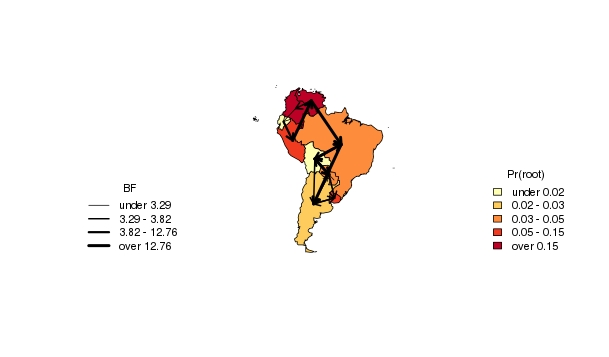
\includegraphics[scale=.450]{FIGURES/O_ss2.jpeg}}%\\
\subfigure[]{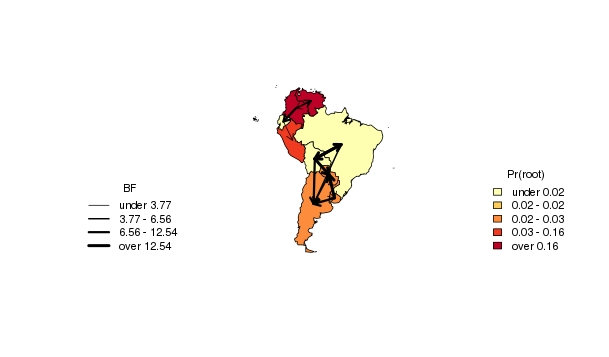
\includegraphics[scale=.450]{FIGURES/O_ss3.jpeg}}
\subfigure[]{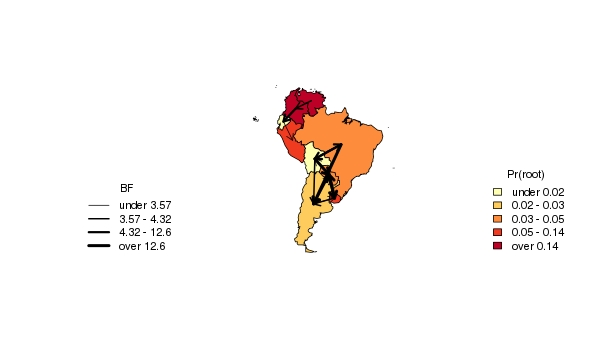
\includegraphics[scale=.450]{FIGURES/O_ss4.jpeg}}%\\
\subfigure[]{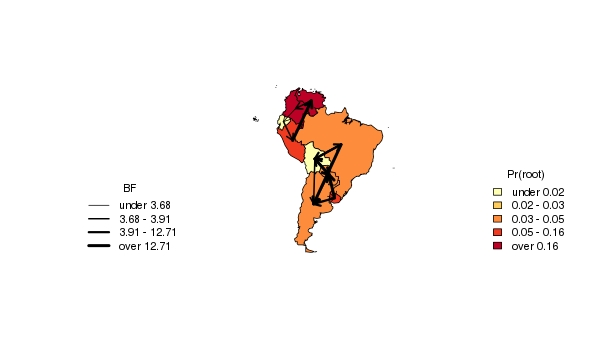
\includegraphics[scale=.450]{FIGURES/O_ss5.jpeg}}
\end{center}
\caption{}
\label{sfig:bssvsO}
\end{figure}
\newpage
\begin{figure}[ht]
\begin{center}
\subfigure[A]{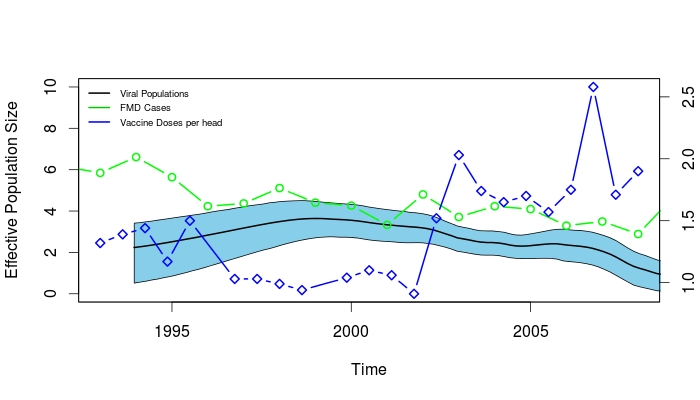
\includegraphics[width=\textwidth]{FIGURES/SFig_A2000sky.jpeg}}
\subfigure[B]{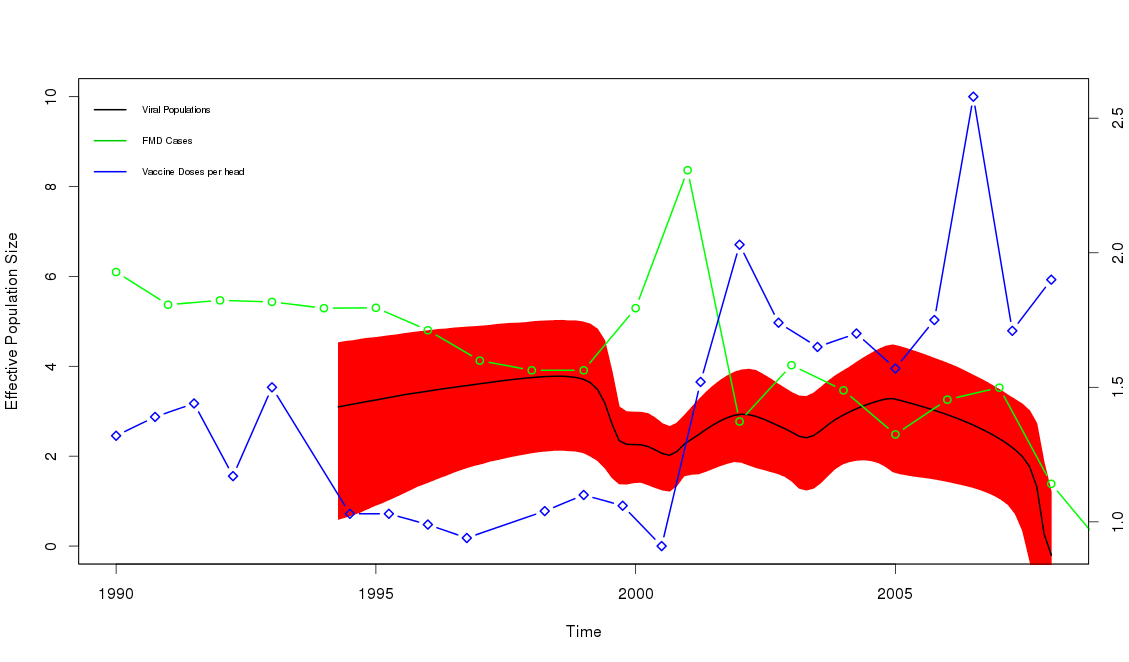
\includegraphics[width=\textwidth]{FIGURES/SFig_O2000sky.jpeg}}\\
\end{center}
\caption{}
\label{sfig:only2000sky}
\end{figure}
\newpage
\begin{table}[ht]
\caption*{\textbf{Table S1. Model selection for tree (coalescent) model and clock for both serotypes.}
ULN= uncorrelated log-normal; UCED = uncorrelated exponential .
Best fitting models (highest log-likelihood) are highlighted in bold.
1- Log-likelihood estimated using Stepping-Stone sampling (SS).}
\begin{center}
\begin{tabular}{cccccc}
\toprule
Serotype	&Coalescent	&Clock	&Log-Likelihood$^{1}$\\
\midrule
A	&Constant	&ULN	&-12285\\
A	&Skyride 	&ULN	&\textbf{-12274}\\
A	&Constant	&UCED	&-12316\\
A	&Skyride 	&UCED	&-12307\\
A       &Skyride       &STRICT &-12308\\
O	&Constant	&ULN	&-8087\\
O	&Skyride 	&ULN	&-8082\\
O	&Constant	&UCED	&-8090\\
O	&Skyride 	&UCED	&\textbf{-8069}\\
O       &Skyride       &STRICT &-8125\\
\bottomrule
\end{tabular}
\end{center}
\begin{flushleft}
\end{flushleft}
\label{stab:treeclockselection}
 \end{table}
 %%%%%%%%%%%%%%%%%%
 %%%%%%%%%%%%%%%%%%
\begin{sidewaystable}[h]
\caption{
\textbf{Spatial signal for FMDV serotypes A and O data sets.} We used Bayesian tip-association significance testing (BaTS) to assess the degree of spatial signal contained in the alignments for both serotypes. 1-Monophyletic clade size}
\begin{tabular}{ccccccc}
\toprule
&\multicolumn{3}{c}{Serotype A} & \multicolumn{3}{c}{Serotype O} \\
MC$^1$ Statistic &Observed mean ( 95\% CI)&Null mean ( 95\% CI)&p-value &Observed mean ( 95\% CI)&Null mean ( 95\% CI)&p-value\\
\midrule
Argentina &12.31 (12.00, 14.00)	&3.45	(2.22, 5.11)	&0.001& 1.00 (1.00, 1.00)&	1.00 (1.00, 1.00)&	1.000\\
Brazil &10.27	(10.00, 11.00)	&2.02 (1.25, 3.00) &0.001& 19.00 (19.00, 19.00)&	2.19 (1.66, 3.03)&	0.001\\
Bolivia &6.00 (6.00, 6.00)	&1.39 (1.00, 2.00)	&0.001&1.00 (1.00, 1.00)&	1.00 (1.00, 1.00)&	1.000\\
Colombia &5.11 (5.00, 6.00)	&1.10  (1.00, 1.99)	&0.001&1.00 (1.00, 1.00)&	1.00 (1.00, 1.00)&	1.000\\
Ecuador &1.00 (1.00, 1.00)	&1.00 (1.00, 1.00)	&1.000&13.00 (13.00, 13.00)&	1.34 (1.00, 2.00)&	0.001\\
Paraguay&-- &-- &--  & 39.40 (31.00, 58.00)& 4.67 (3.43, 6.39)&0.001\\
Peru&1.00 (1.00, 1.00)	&1.02 (1.00, 1.00)&1.000&1.00 (1.00, 1.00)&1.01 (1.00, 1.00)&1.000\\
Uruguay &5.11 (5.00, 7.00)	&1.50	(1.00, 2.03)	&0.001&4.00 (4.00, 4.00)&	1.06 (1.00, 1.32)&	0.001\\
Venezuela&1.82 (1.00, 2.00)	&1.02 (1.00, 1.08)	&0.010&6.00 (6.00, 6.00)&	1.28 (1.00, 2.00)&	0.001\\
\bottomrule
\end{tabular}
\begin{flushleft}
\end{flushleft}
\label{tab:BaTS}
\end{sidewaystable}
%%%%%%%%%%%%

\begin{table}[h]
\caption*{ {{\bf Table S2 Parameter estimation using the complete and without Argentina data sets for serotype A.}} To assess the impact of the overrepresentation of Argentina in our sample we removed all sequence from this location and reestimated parameters.
1- All 131 sequences were used. 2- Time to most recent common ancestor. 3- Codon positions $1$, $2$ and $3$. }
\begin{center}
\begin{tabular}{ccc}
\toprule
Parameter	&Complete$^{1}$	&Without Argentina\\
\midrule
TMRCA$^{2}$	&76.40 (69.48-83.65)	&82.31 (72.40-92.81)\\
CP1$	^{3}$	&0.65 (0.54-0.76)	&0.62 (0.51-0.75)\\
CP2	&0.46 (0.37-0.58)	&0.41 (0.31-0.53)\\
CP3	&1.87 (1.74-2.00)	& 1.95 (1.81 -2.09)\\
Rate ($\times 10^{-3}$)	&4.14 (3.39-4.98)	&3.46 (2.82-4.11)\\
\bottomrule
\end{tabular}
\end{center}
\label{tab:SB_A}
 \end{table}


%%%%%%%%%
%%%%%%%%%
\begin{table}[h]
\caption{ {{\bf Parameter estimation using the complete and without Ecuador data sets for serotype O.}} To assess the impact of the overrepresentation of Ecuador (90 sequences) our sample we removed all sequence from this location and reestimated parameters.
1- All 167 sequences were used. 2- Time to most recent common ancestor. 3- Codon positions $1$, $2$ and $3$.
}
\begin{center}
\begin{tabular}{ccc}
\toprule
Parameter	&Complete$^{1}$	&Without Ecuador\\
\midrule
TMRCA$^{2}$	&21.25 (19.20-23.60)	&22.65 (17.6-29.5)\\
CP1$^{3}$	&0.51 (0.39-0.63)	&0.51 (0.39-0.64)\\
CP2	&0.53 (0.39-0.69)	&0.42 (0.29-0.59)\\
CP3	&1.94 (1.78-2.10)	& 2.05 (1.87 -2.21)\\
Rate ($\times 10^{-2}$)	&1.11 (0.91-1.32)	&0.91 (0.63-1.21)\\
\bottomrule
\end{tabular}
\end{center}
\label{tab:SB_O}
 \end{table}

%%%%
%%%%
\newpage
\begin{sidewaystable}[ht]
\medskip
\begin{minipage}{\textwidth} 
\begin{center}
\caption{ {{\bf 'Equal downsampling' experiment for serotype A.}} 
Five random downsampled subsamples were obtained and used for parameter inference.
1-- $\times 10^{-3}$. 2 -- $\times 10^{-2}$. 3-- Probabily at root node.}
\begin{tabular}{ccccc}
\toprule
Subsample	&mean subs. rate$^{1}$ (95 \% BCI)	&TMRCA (95 \% BCI)	&mean migration rate$^{2}$  (95 \% BCI)	&Root (Pr$^{3}$)\\
\midrule
1	&4.21 (3.43-5.05)	&78.97 (71.21-86.82)	&2.63 (1.34-4.08)	&Brazil (0.78)\\
2	&4.25 (3.44-5.07)	&79.64 (71.49-88.04)	&2.54 (1.28-3.98)	&Brazil (0.79)\\
3	&4.12 (3.38-4.94)	&77.74 (70.26-85-86)	&2.49 (1.27-3.88)	&Brazil (0.81)\\
4	&4.12 (3.41-4.82)	&77.60 (69.41-85.88)	&2.44 (1.21-3.85)	&Brazil (0.87)\\
5	&4.19 (3.49-4.93)	&78.28 (70.23-86.96)	&2.66 (1.31-4.11)	&Brazil (0.82)\\
\bottomrule
\end{tabular}
\label{tab:ED_A}
\end{center}
\end{minipage}
\end{sidewaystable}

%%%%
%%%%
\newpage
\begin{sidewaystable}[ht]
\medskip
\begin{minipage}{\textwidth}
\begin{center}
 \caption{ {{\bf 'Equal downsampling' experiment for serotype O.}} Five random downsampled subsamples were obtained and used for parameter inference.
1-- $\times 10^{-2}$. 2--  Probabily at root node.}
\begin{tabular}{ccccc}
\toprule
Subsample	&mean subs. rate$^{1}$ (95 \% BCI)	&TMRCA (95 \% BCI)	&mean migration rate$^{1}$ (95 \% BCI)	&Root (Pr$^{2}$)\\
\midrule
1	&1.11 (0.86-1.37)	&20.27 (18.45-21.95)	&8.48 (3.91-13.59)	&Colombia (0.98)\\
2	&0.865 (0.62-1.11)	&22.40 (19.78-25.31)	&8.74 (3.84-14.28)	&Colombia (0.93)\\
3	&0.94 (0.68-1.21)	&21.91 (19.46-24.56)	&8.72 (4.03-14.17)	&Colombia (0.93)\\
4	&0.84 (0.62-1.18)	&22.54 (19.80-25.45)	&8.43 (3.77-13.67)	&Colombia (0.99)\\
5	&0.88 (0.63-1.13)	&22.33 (19.55-25.26)	&8.58 (3.89-13.18)	&Colombia (0.92)\\

\bottomrule
\end{tabular}
\label{tab:ED_O}
\end{center}
\end{minipage}
\end{sidewaystable}
%%%%
%%%%
\end{document}
